
\documentclass[conference]{IEEEtran}
% Add the compsoc option for Computer Society conferences.
%
% If IEEEtran.cls has not been installed into the LaTeX system files,
% manually specify the path to it like:
% \documentclass[conference]{../sty/IEEEtran}





% Some very useful LaTeX packages include:
% (uncomment the ones you want to load)


% *** MISC UTILITY PACKAGES ***
%
%\usepackage{ifpdf}
% Heiko Oberdiek's ifpdf.sty is very useful if you need conditional
% compilation based on whether the output is pdf or dvi.
% usage:
% \ifpdf
%   % pdf code
% \else
%   % dvi code
% \fi
% The latest version of ifpdf.sty can be obtained from:
% http://www.ctan.org/tex-archive/macros/latex/contrib/oberdiek/
% Also, note that IEEEtran.cls V1.7 and later provides a builtin
% \ifCLASSINFOpdf conditional that works the same way.
% When switching from latex to pdflatex and vice-versa, the compiler may
% have to be run twice to clear warning/error messages.






% *** CITATION PACKAGES ***
%
% \usepackage{cite}
% cite.sty was written by Donald Arseneau
% V1.6 and later of IEEEtran pre-defines the format of the cite.sty package
% \cite{} output to follow that of IEEE. Loading the cite package will
% result in citation numbers being automatically sorted and properly
% "compressed/ranged". e.g., [1], [9], [2], [7], [5], [6] without using
% cite.sty will become [1], [2], [5]--[7], [9] using cite.sty. cite.sty's
% \cite will automatically add leading space, if needed. Use cite.sty's
% noadjust option (cite.sty V3.8 and later) if you want to turn this off.
% cite.sty is already installed on most LaTeX systems. Be sure and use
% version 4.0 (2003-05-27) and later if using hyperref.sty. cite.sty does
% not currently provide for hyperlinked citations.
% The latest version can be obtained at:
% http://www.ctan.org/tex-archive/macros/latex/contrib/cite/
% The documentation is contained in the cite.sty file itself.





\usepackage[dvips]{graphicx}
\graphicspath{{./images/}}
\DeclareGraphicsExtensions{.eps,.bmp}

\hyphenation{op-tical net-works semi-conduc-tor}


\begin{document}
%
% paper title
% can use linebreaks \\ within to get better formatting as desired
\title{An Analysis of high speed Interconnect Technology: Quickpath
Interconnect, PCI-Express and HyperTransport}


% author names and affiliations
% use a multiple column layout for up to three different
% affiliations
\author{\IEEEauthorblockN{James Swaro}
\IEEEauthorblockA{School of Electrical Engineering\\ and Computer Science\\
Ohio University\\
Athens, Ohio 45701--3241\\
Email: js311004@ohio.edu}
}

% make the title area
\maketitle


\begin{abstract}
\label{sec:abstract}
%\boldmath
This paper serves to evaluate Quickpath Interconnect, HyperTransport and PCI
Express as high speed interconnect technologies. A comparison will be made,
highlighting the advantages and disadvantages of each technology. Quickpath
Interconnect is a proprietary technology developed by Intel to increase the
available bandwidth between the CPU and the north bridge. PCI-Express is
technology managed by PCISIG that serves as a replacement for PCI and PCI-X,
while also attempting to be a consumer grade high speed motherboard--level
interconnect. HyperTransport is an interconnect technology designed by AMD
designed to function as a direct to CPU interconnect for I/O devices. This paper
will summarize each technology in detail, comparing the advantages and
disadvantages of each technology as well as a brief synopsis about how each
interconnect functions. 
\end{abstract}
% IEEEtran.cls defaults to using nonbold math in the Abstract.
% This preserves the distinction between vectors and scalars. However,
% if the conference you are submitting to favors bold math in the abstract,
% then you can use LaTeX's standard command \boldmath at the very start
% of the abstract to achieve this. Many IEEE journals/conferences frown on
% math in the abstract anyway.

% no keywords




% For peer review papers, you can put extra information on the cover
% page as needed:
% \ifCLASSOPTIONpeerreview
% \begin{center} \bfseries EDICS Category: 3-BBND \end{center}
% \fi
%
% For peerreview papers, this IEEEtran command inserts a page break and
% creates the second title. It will be ignored for other modes.
\IEEEpeerreviewmaketitle



\section{Introduction}
\label{sec:intro}
% no \IEEEPARstart
As computers are increasing in performance in the areas of memory, networking,
storage and processing, the interconnects must also improve. The improvement of
interconnects comes as a necessity so that overall systems performance does not
become hindered as other components improve. Such components include the
processor, memory and I/O devices which are constantly increasing in bandwidth,
the interconnects that connect these devices must also improve. 
In modern computers, the north bridge typically serves as the interconnect fabric
between the south bridge, graphics and memory hub to the processor. The
south bridge is responsible for communicating with slower I/O devices and the
north bridge. However, in high performance computing, it can be easy to find
that the bandwidth required to perform certain tasks can exceed that of the
available bandwidth. This is where it is often necessary to look at faster
interconnect technologies such as HyperTransport, QPI or PCI-Express. 

Each technology addresses the need for faster I/O with the CPU in a different
way. The way in which this is done can vary greatly with each technology and
with differing results. This paper will address the differences between each
technology and examine the advantages versus the disadvantages of each
technology to provide an unbiased analysis. 

\section{QuickPath Interconnect}
This section will describe the Intel QuickPath Interconnect in detail,
highlighting the advantages and disadvantages. It will also cover a brief
overview of how the protocol works in brief detail. 
\subsection{Overview}
QuickPath Interconnect is a proprietary interconnect technology developed by
Intel in response to the development of HyperTransport. Increasing
CPU speed and bottlenecks at the front-side bus are also attributed to the
development of this technology. Unlike HyperTransport and PCI-Express, QuickPath
Interconnect serves to replace the front-side bus instead of complementing it.
QuickPath is a high speed point-to-point
interconnect\cite{intelQPIintro}.\footnote{Image for Figure \ref{fig:qpi:fabric} belongs to Lost Circuits 
\\$http://www.lostcircuits.com/cpu/intel_i7/qpi1.jpg$}
\footnote{Image for
Figure \ref{fig:qpi:diagram} belongs to XBit Laboratories,
\\$http://www.xbitlabs.com/images/news/2009-05/intc_beckton_platform.png$}
QPI is known to operate at 4.8GT/s to 6.4GT/s or 19.2GB/s to 25.6GB/s. 
\begin{figure}[!t]
	\begin{center}
		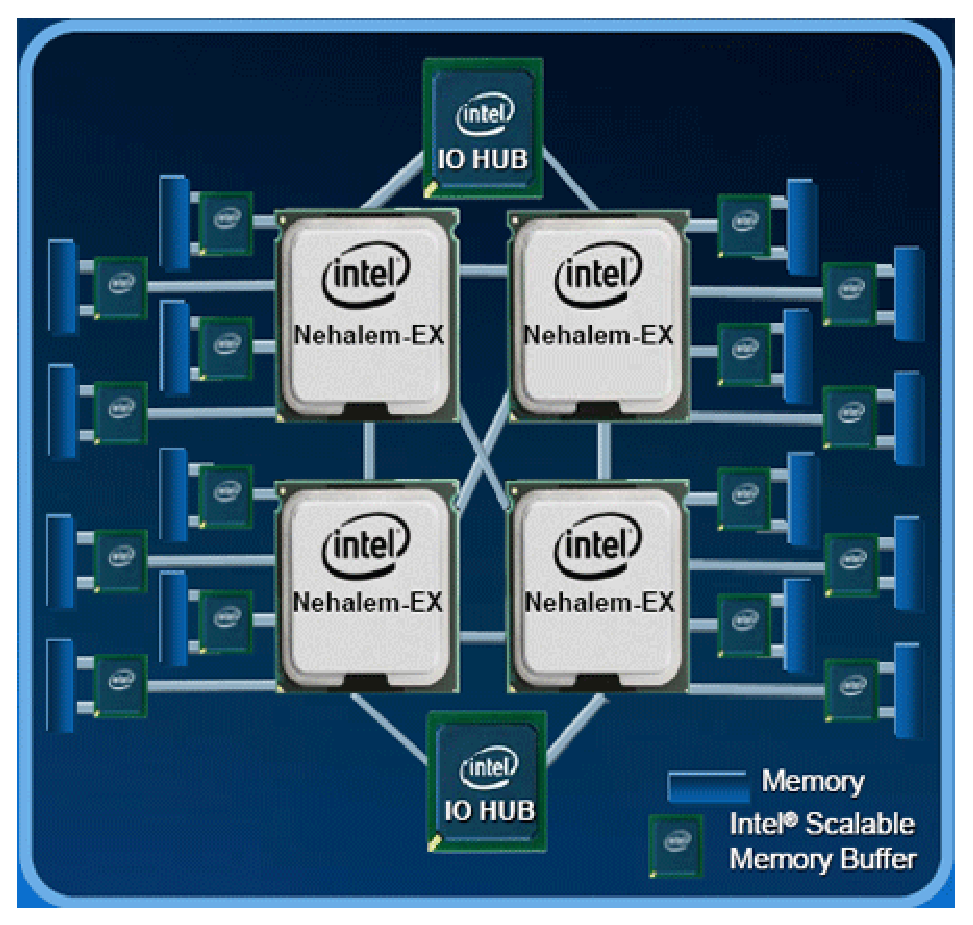
\includegraphics[scale=.35]{qpiDiagram}
	\end{center}
	\caption{An example of a QPI interconnect.}
	\label{fig:qpi:diagram}
\end{figure}

\begin{figure}[!t]
	\begin{center}
		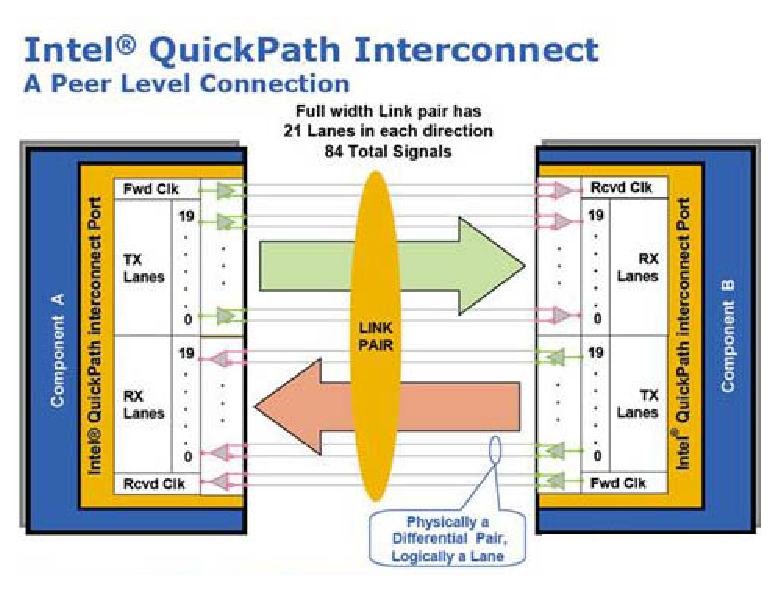
\includegraphics[scale=.6]{qpiFabric}
	\end{center}
	\caption{The connection between two components connected by
	QPI.}
	\label{fig:qpi:fabric}
\end{figure}


\subsection{How does it operate?}
QPI links are sets of twenty differential signal pairs. The differential
signaling helps to alleviate noise, reducing error and increasing throughput
when errors are avoided. Each pair consists of two uni-directional links,
allowing for traffic in both directions simultaneously. 
QPI is implemented at five different layers\cite{intelQPIintro}. This can be
observed by Figure \ref{fig:qpi:layers}. The physical layer sends packets along
each link at 20b phit sizing. The data link layer sends packets along each link
at 80b flit sizing. The routing layer of QPI wraps each segment in a small
header for addressing as follows:

\bigskip

\begin{quote}
The routing layer sends a 72-bit unit consisting of an 8-bit
header and a 64-bit payload. The header contains the destination and the message type.
When the routing layer receives a unit, it examines its routing tables to
determine if the unit has reached its destination. If so it is delivered to the
next-higher layer. If not, it is sent on the correct outbound QPI. On a device
with only one QPI, the routing layer is minimal. For more complex
implementations, the routing layer's routing tables are more complex, and are
modified dynamically to avoid failed QPI links.\footnote{This was taken
directly from the wikipedia page as not much information is available about how
QPI routes.}
\end{quote}

The transport layer of QPI is usually architecture dependent, often not defined
until the final product is in place. This seems to be the most inflexible part
of QPI\cite{intelQPIintro}.

\begin{figure}[!t]
	\begin{center}
		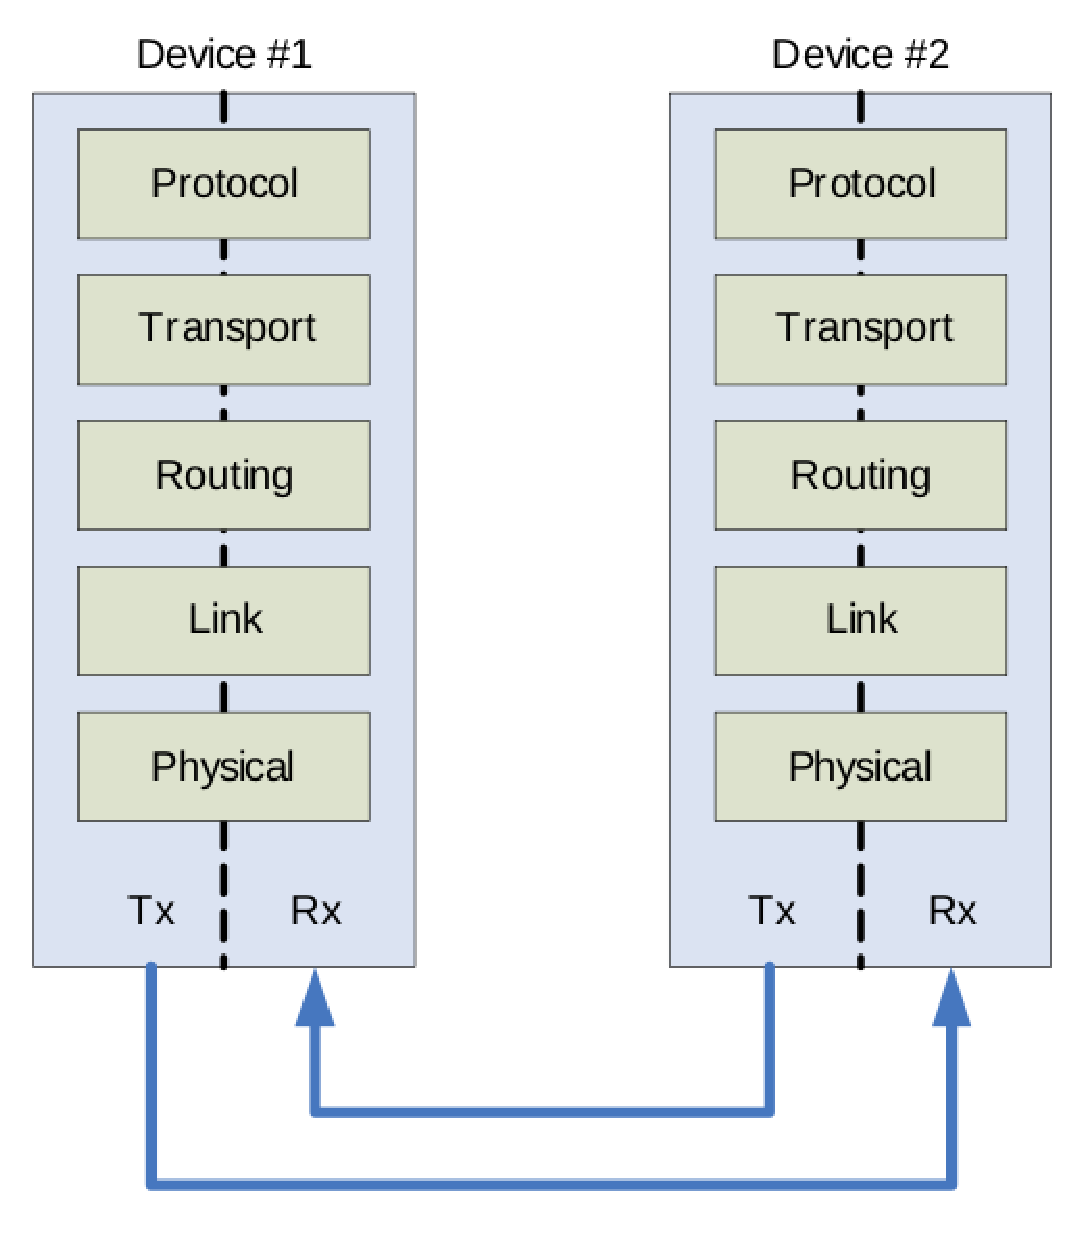
\includegraphics[scale=.25]{qpiLayers}
	\end{center}
	\caption{QPI layering model}
	\label{fig:qpi:layers}
\end{figure}
\subsection{Advantages}
At the physical layer, special logic is in place to serve as a fail-safe in
cases where QPI will reduce the number of links utilized when one fails so that
data will continue to be sent as quickly as possible while reducing
retransmissions. Additionally, QPI offers lane/polarity reversal, data recovery,
deskew circuits and waveform reversal for additional
stability\cite{intelQPIintro}. CRC error detection is also provided , including
link level retransmission capability, hot-plugging support and link-self
healing. 

QPI also defined up to fourteen  different message classes so that traffic can
be prioritized. Currently , only six of them are defined as of the time that the
QPI white paper was written\cite{intelQPIintro}. QPI also uses a cache coherency
protocol to keep memory coherent during operation. 
\subsection{Disadvantages}

One of the more noticeable disadvantages that I observed was that each flit has
eight bits reserved for CRC, accounting for ten percent of every flit sent. This
high level of overhead is detrimental to the actual throughput.\footnote{Not
many more examples of disadvantages were found as information on QPI seemed to
be limited.}

\section{HyperTransport}
\label{sec:ht}
This section will describe the HyperTransport interconnect protocol in detail,
highlighting the advantages and disadvantages. It will also cover a brief
overview of how the protocol works in brief detail. 

\subsection{Overview}
\label{subsec:ht:over}
HyperTransport was originally designed to support to need simplify high-speed
data traffic between memory, I/O or the processor. The first
specification, HyperTransport 1.03 defined a bandwidth of up
to 12.8 GB/s aggregate bandwidth.\cite{htWhitePaper} HyperTransport 2.0
supports 22.4 GB/s aggregate bandwidth and the newest specification,
HyperTransport 3.10 supports up to 25.6GB/s unidirectional.

HyperTransport is referred to as a ``mezzanine connector from a system's main
processor or memory controller to another I/O, often a PCI bus, within the
system, perhaps for additional chip or component.''\cite{paulson2003ins} As I
have read, HyperTransport is often directly connected to the CPU and functions
similarly to the north bridge but only for high speed I/O devices. 

HyperTransport is a point-to-point link technology that uses two separate
point-to-point links for bi-directional traffic, up to speeds of 51.2GB/s
bidirectional. A set of HyperTransport links can be seen in Figure
\ref{fig:htLinks}. 

\begin{figure}[!t]
	\begin{center}
		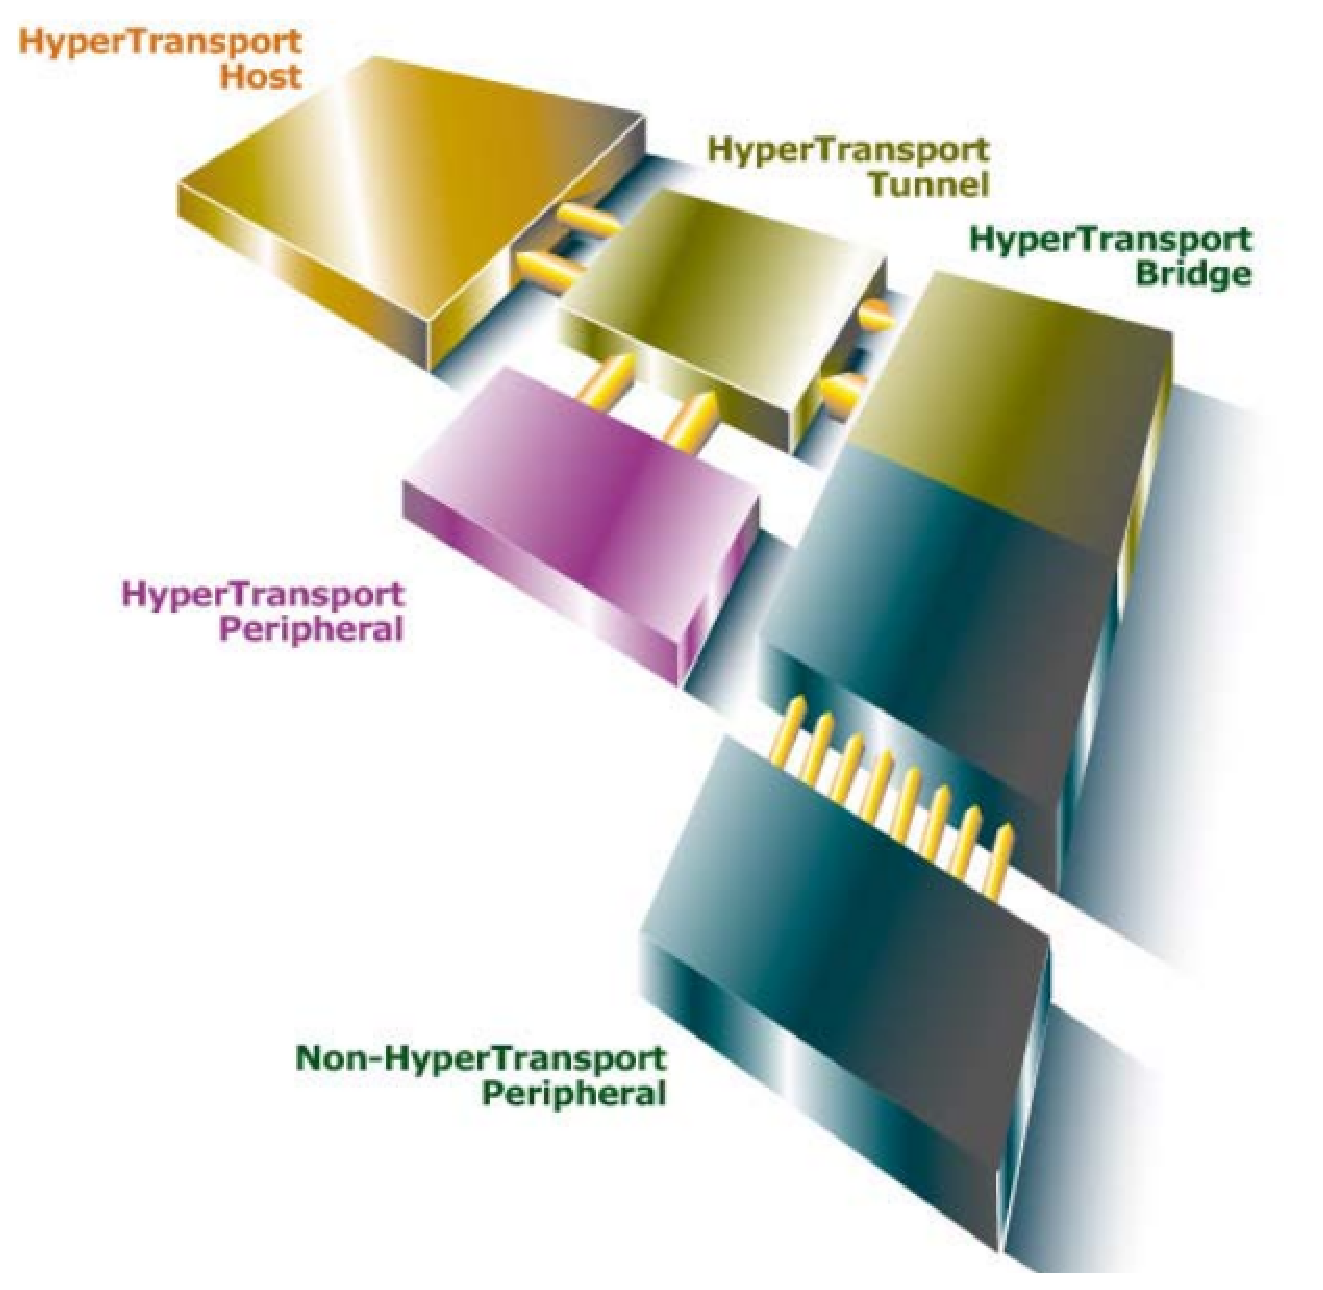
\includegraphics[scale=.35]{htLinks}
	\end{center}
	\caption{
	 The HyperTransport Link consists of at least one host (often a
	 HyperTransport-enabled CPU) and one tunnel/endpoint. A tunnel enables the
	 HyperTransport link to be passed from one HyperTransport-enabled device to
	 another in daisy-chain fashion.
	\cite{htWhitePaper}\label{fig:htLinks}}
	\label{fig:ht:packet}
\end{figure}

HyperTransport is also a very low latency protocol with a very high bandwidth
capability. It is achieved by the following:\cite{duato2009extending}

\begin{itemize}
  \item Minimizing packet overhead
  \item Eliminating control and command signals needed by other protocols
  \item Reducing crosstalk and interference
\end{itemize}

HyperTransport is however primarily a host-to-host or host-to-I/O protocol.
This can be observed in Figure \ref{fig:ht:diagram}. It does not see that same
benefits as it is expanded to larger scale environments. HyperTransport interconnects can function as a replacement of the
north bridge,  a multiprocessor interconnect or a switch bus. 
HyperTransport has four different protocol versions. HT protocol 1.x and 2.0
are clock-forwarded interface types. The links are considered to be
uni-directional reliable links, operating at a clock speed of 200 MHz to 3.2Mhz(HT3.1).
HyperTransport 3.0 and up is not considered to be reliable due to the use of
data recovery techniques.\cite{holden2006latency}. However, it can be shown that
the rate of bit errors is low. 

HyperTransport was designed to be an extremely low latency protocol. With this
in mind, the designers created HyperTransport in such a way as to minimize the
latency within the physical, data link and transaction layer. This is due to
the low amount of packet overhead generated by the headers in a HT packet and a
skew-constrained PCB.

\begin{figure}[!t]
	\begin{center}
		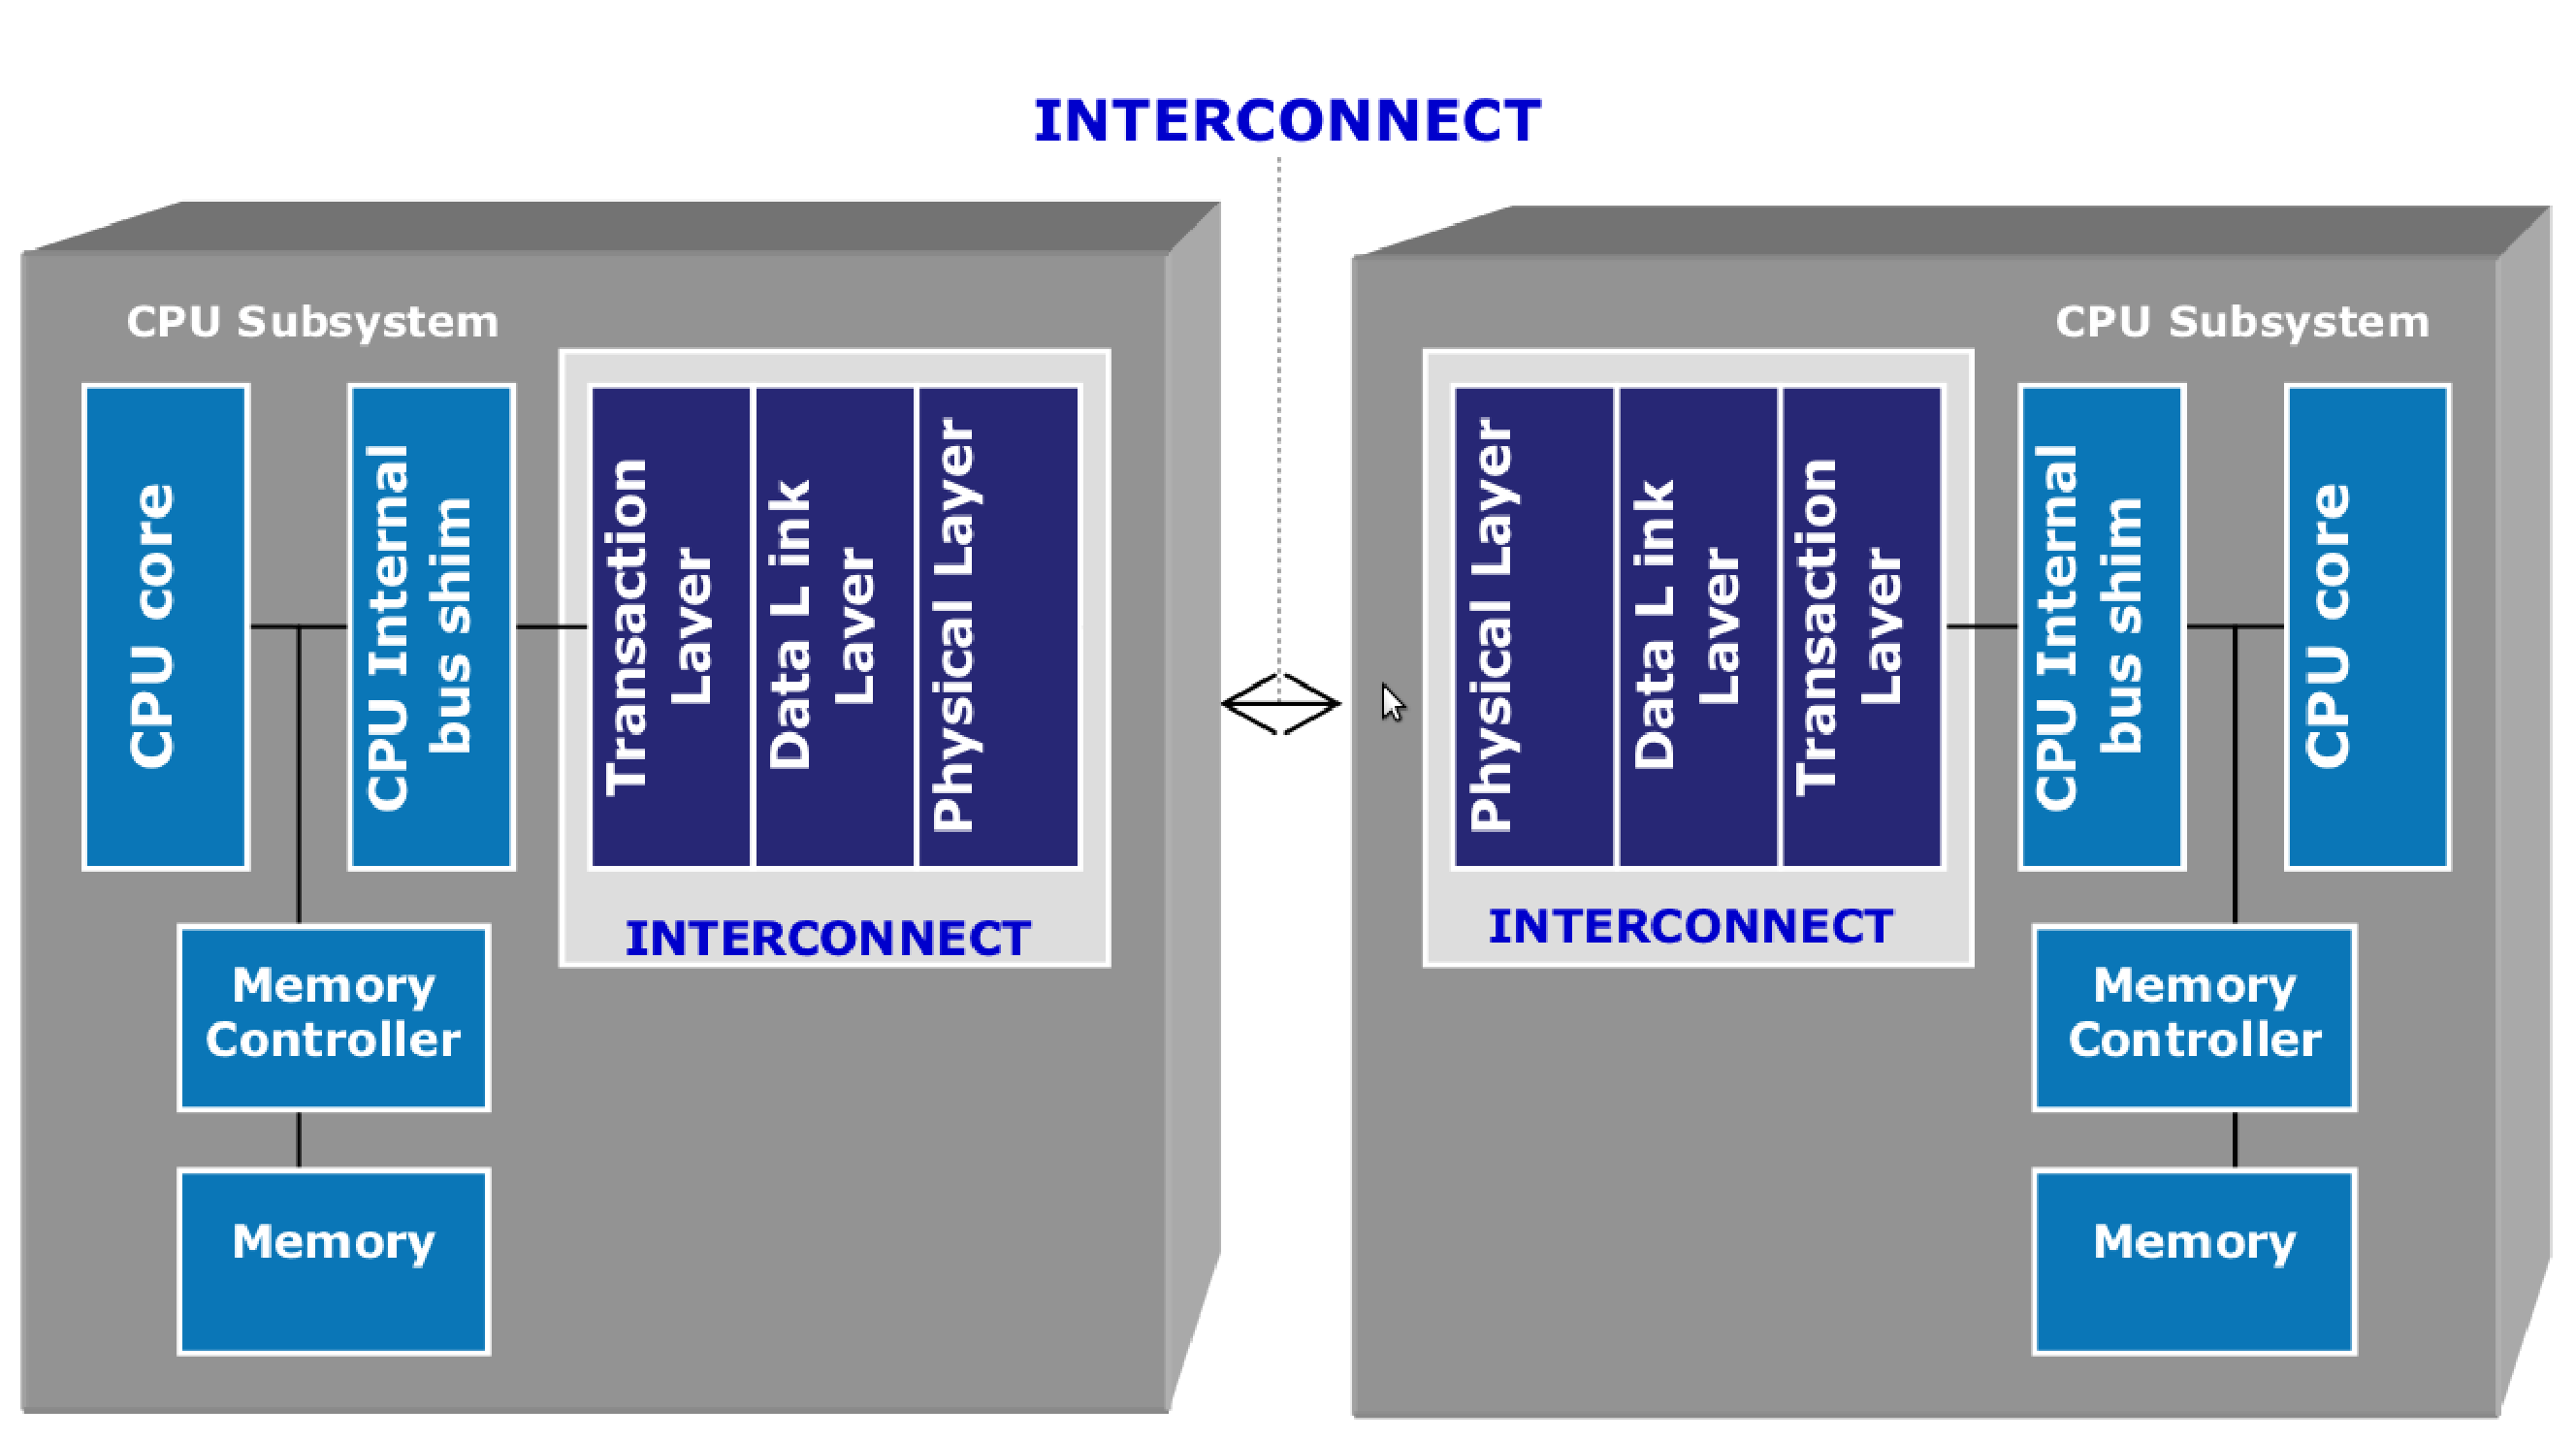
\includegraphics[scale=.15]{htDiagram}
	\end{center}
	\caption{point-to-point visualization of a
	HyperTransport link.\cite{holden2006latency}.}
	\label{fig:ht:diagram}
\end{figure}

\subsection{How does it operate?}
\label{subsec:ht:oper}


HyperTransport is often connected directly to the CPU. It serves as a bridge
between high speed I/O devices and the CPU providing a high bandwidth channel for
multiple devices to use to communicate. Each devices is connected to the HT bus
through a daisy chain. Up to thirty-two devices to be connected to any single
daisy chain. The daisy chain operates by allowing a device to take up a set of lines,
of which do not have to match the number of lines taken by other devices. For
example, a single I/O devices connected to the HT unit, can utilize two lines,
while another device can use eight. 

The HT protocol maintains the high speed by eliminating overhead from packets
transferred. The read packets of a HT link only have an overhead of eight bytes
while the write packets have an overhead of twelve bytes. This minimal amount of
bytes reserved for overhead results in a large boost in performance. This can be
observed in Figure \ref{fig:ht:packet}.

\begin{figure}[!t]
	\begin{center}
		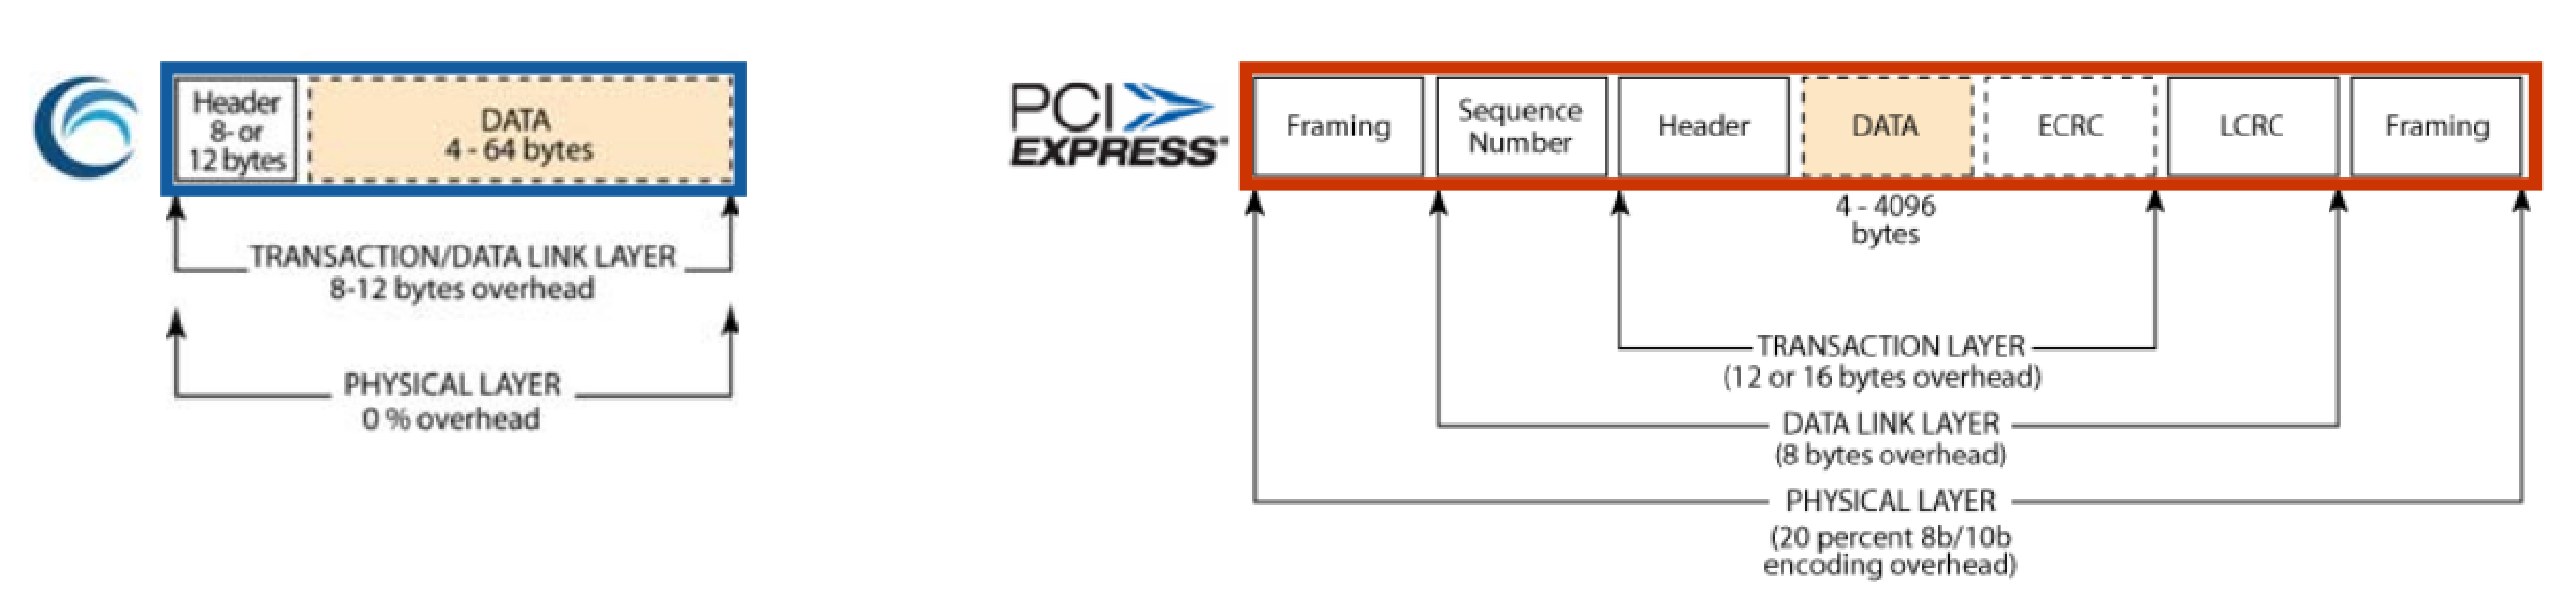
\includegraphics[scale=.2]{htPacket}
	\end{center}
	\caption{A comparison between a HyperTransport packet and a PCI-Express
	packet.\cite{holden2006latency}}
\end{figure}
 
\subsection{Advantages}
\label{subsec:ht:advant}
HyperTransport is designed with many key advantages in mind. The interface
design for HyperTransport 1.x and 2.0 is considered to be inherently reliable.
This improves throughput as less effort is expended attempting to re-transmit
lost data. It is further improved upon by looking at the bit error ratio.
HyperTransport consortium claims that the bit-error-ratio of the system is
often 10-15 or better.\cite{holden2006latency} This allows the designers to use
simple error detection instead of complicated and often expensive in terms of either latency or
bandwidth loss. 

Low latency is a key design advantage that was considered during the development
of HyperTransport. With that in mind, Priority Request Interleaving is a feature
specific to HyperTransport that allows for data to be halted and control packets
to be inserted in the case where a control packet may need to be transmitted
immediately. This is significant in that PRI can reduce latency considerably,
usually in response to a cache-miss or similar events\cite{holden2006latency}.

Consider the following event given from the Latency Comparison paper from
the HyperTransport Consortium:

\bigskip

\begin{quote}
While data transfer 1 is underway between peripheral B and the
host, the need arises for peripheral A to start a data transfer from the host. Without PRI, transfer 2 would have to wait
until transfer 1 completes and, should transfer 1 be the answer to a cache miss, for instance,
latency for transfer 2 would become prohibitive. With PRI, a control packet is promptly
inserted within transfer 1's data stream, instructing the link to initiate data transfer 2 on the
other link channel concurrently with the completion of data transfer 1. This mechanism,
unique to HyperTransport technology, greatly reduces latency of HyperTransport-based
systems.\cite{holden2006latency}
\end{quote}

\bigskip

HyperTransport also does split-phase transactions that allow the I/O device to
continue on with other tasks. In addition, HyperTransport does not require framing or coding at the physical
layer, CRC is performed every 512 bytes instead of a packet by packet basis and
no data link layer packet overhead is present.

\subsection{Disadvantages}
\label{subsec:ht:disadv}
Unfortunately, HyperTransport does not support hardware error recovery at the
link layer. The following is a list of things that HyperTransport cannot do
well:

\begin{itemize}
  \item Cannot do global device addressing beyond 32 nodes.
  \item Efficient routing in scalable network topologies
  \item Scalable congestion management mechanisms
  \item Dynamic reconfiguration of routing information
\end{itemize}

The above items are relevant for clustering HyperTransport devices in medium to
large clusters of processing nodes\cite{duato2009extending}. 

\section{PCI-Express}
This section will describe the PCI Express in detail,
highlighting the advantages and disadvantages. It will also cover a brief
overview of how the protocol works in brief detail. 
\subsection{Overview}
PCI-Express was designed by PCISIG as an upgrade to the old PCI and PCI-X
technologies. As the necessity for higher bandwidth to support I/O devices rose, the need for faster interconnect
initiated the design of PCI-Express. PCI-Express is a switched, serial
interconnect technology. PCI-Express serves as a switch environment to a
plethora of I/O devices ranging from graphics to high speed I/O devices like
networking interfaces. The architecture is layered similarly to the OSI
technology and it is designed to be compatible with copper, optical or other
forms of media\cite{paulson2003ins}. PCI-Express allows for hot-plugging and
power management. Originally known as 3GIO, PCI-Express has been in development
for a long time with PCI-Express 3.0 being the latest standard with PCI-Express
4.0 under development and slated for 2014/15 specification release date. 

Functionally, PCI and PCI-Express are both bus topologies. PCI is a shared bus
technology where PCI-Express is a point-to-point bus technology where each
device has a separate serial link connecting it to the root complex of the PCI
Express bus.\cite{budruk2004pci} The structure of a PCI-Express interconnect can
be observed in Figure \ref{fig:pci:diagram}.

\begin{figure}[!t]
	\begin{center}
		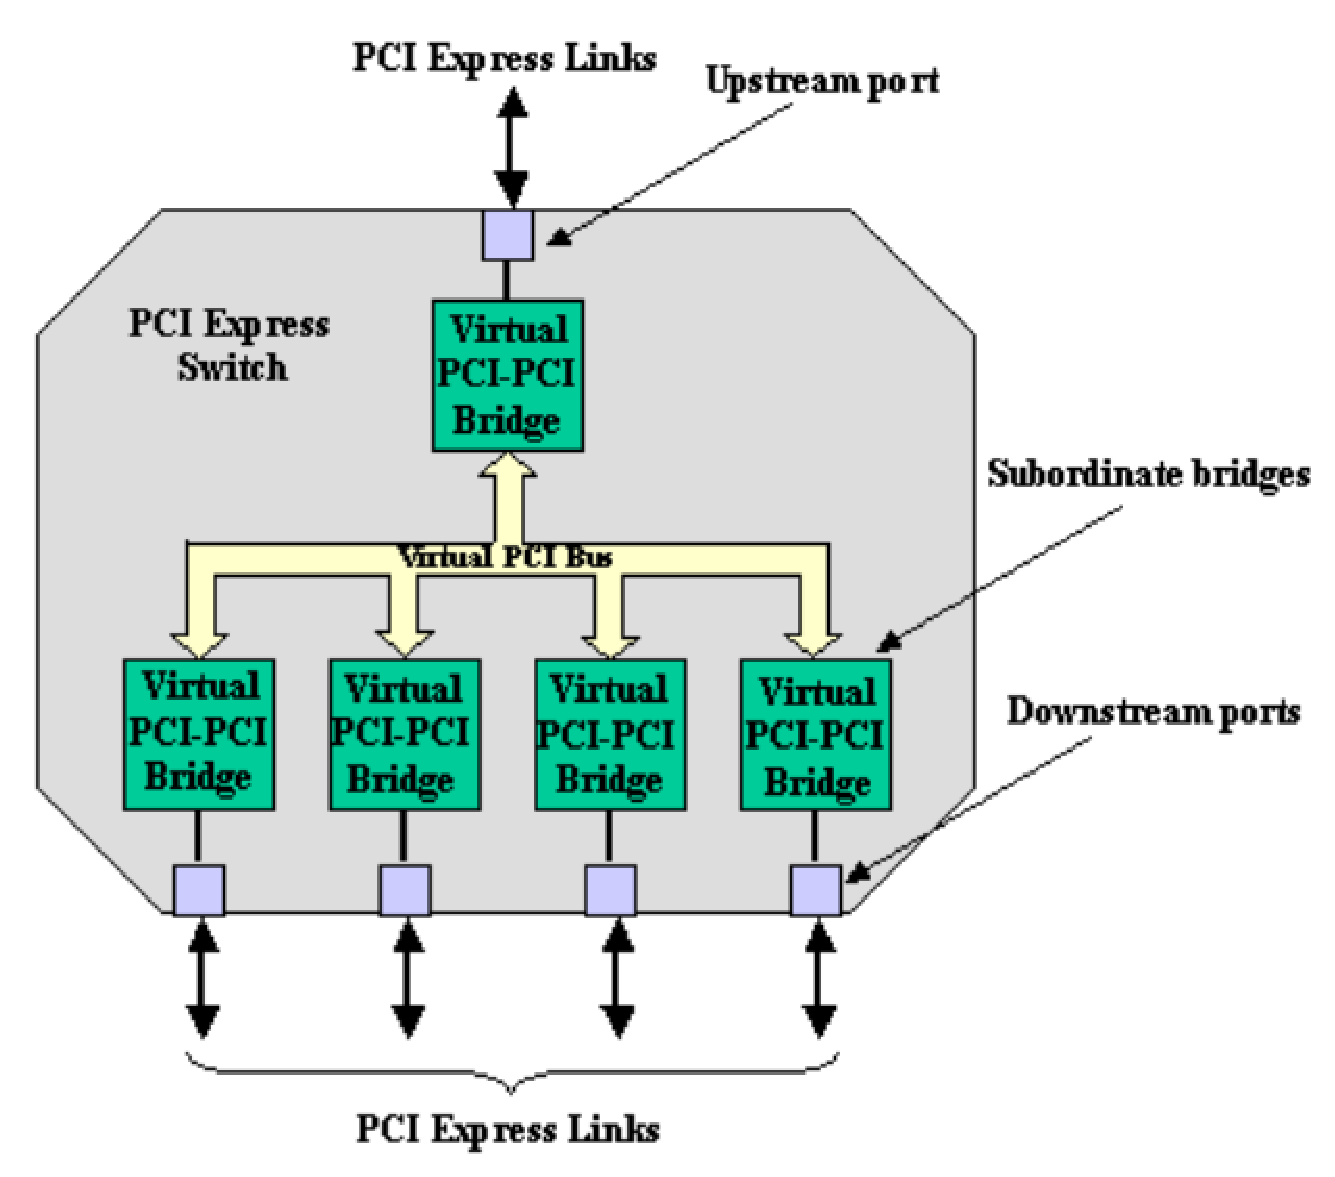
\includegraphics[scale=.4]{pciDiagram}
	\end{center}
	\caption{PCI Express Architecture as it functions as a switching fabric
	between high speed I/O devices.\cite{mayhew2003pci}}
	\label{fig:pci:diagram}
\end{figure}

\begin{figure}[!t]
	\begin{center}
		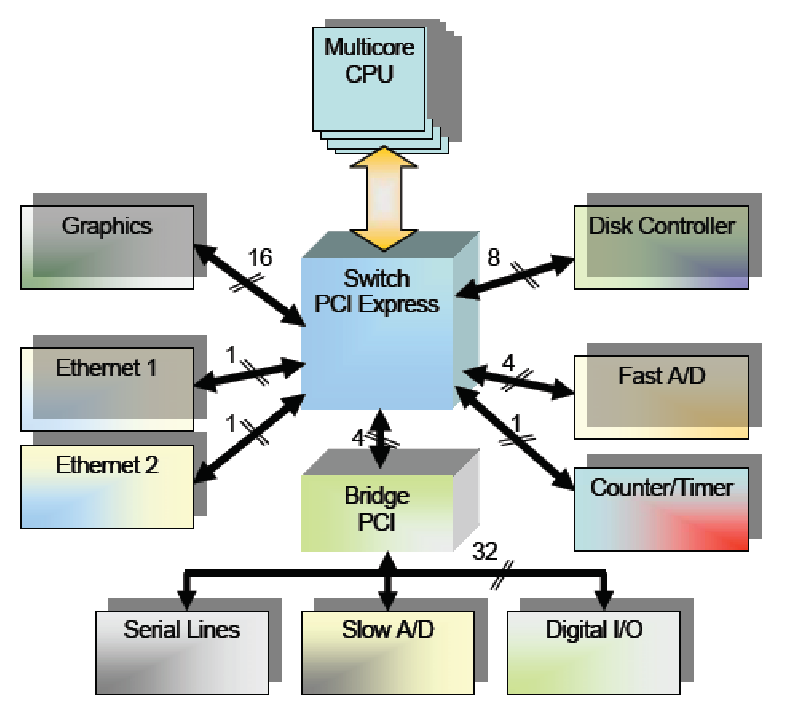
\includegraphics[scale=.6]{pciFabric}
	\end{center}
	\caption{PCI Express Fabric representation}
	\label{fig:pci:fabric}
\end{figure}

The PCI-Express link between any two devices can consist of one to thirty-two
lanes. A lane is a set of TX/Rx Pair of lines connecting two devices, creating
a full duplex environment in which packets are transported. To expand upon this,
PCI-Express also allowed the data to be delivered in parallel on connections in
which more than one lane exists.The current specification, PCI-Express 3.0 can
do 8.0GT/s or 16GB/s in a sixteen-lane environment. 

PCI-Express is considered to be an ``inside of the box'' I/O solution while
other technologies such as Infiniband can be used to connect high speed devices
or cluster interconnects.

\subsection{How does it operate?}
\label{sub:pci:oper}
PCI-Express is a multi-drop, parallel bus topology. Each interconnect contains a
Host bridge and has several endpoints to connect I/O
devices\cite{bhatt2003creating}. PCI-Express functions on three different layers
of the OSI model, mapped to the Physical layer, Data link layer and Transaction
layer. The Data transmission layer is responsible for sending all control
messages, interrupts and data for the interconnect. Data is interleaved such
that each successive byte is sent down each successive lane available to the
connection. This is how the connection between devices is parallelized to
increase bandwidth between devices. 

The data is encoded in a 8b to 10b transfer
encoding, creating a twenty percent overhead at the Physical layer. An
improvement was made in PCI-Express 3.0 such that the data was encoded in a 128b
to 130b transfer encoding, decreasing the overhead incurred at the Physical
layer of the protocol.

The data link layer was designed to ensure the reliable deliver of packets
between two endpoints using ACK/NACK and a sliding window. PCI-Express also
utilizes a credit-based flow control that always ensures that there is space for
the packets sent in the next hop of the path.

The Transaction layer utilizes split transactions similar to HyperTransport
allowing I/O devices to continue other tasks while waiting for read and write
requests to complete. This layer will generate the read and write requests and
pass down to the data link layer for the addition of sequence information and
CRC checking. 

\subsection{Advantages}
\label{sec:pci:advant}

There are many advantages to using PCI-Express as an interconnect. PCI-Express
uses a credit-based flow control so that packets are only sent when space is
available for them in the receiving buffer. This helps to eliminate
retransmissions and loss of bandwidth due to retransmissions. PCI-Express also
attempts the concept that there is no notion of a system boundary within
PCI-Express\cite{mayhew2003pci}. PCI-Express also allows hot-plugging and
reconfiguration of endpoints on the fly, allowing the interconnect to be
flexible with little pre-configuration necessary. Similar to HyperTransport,
PCI-Express also supports packet stomping and data
poisoning\cite{holden2006latency}. 

PCI-Express is relatively low cost and easily scalable, making it suitable for
many different types of computing applications. It also provides end-to-end CRC
checking to reduce transmission errors. PCI-Express also offers scrambling to
reduce electro-magnetic interference at the physical layer, providing additional
benefit not seen in HyperTransport. Each packet sent via PCI-Express has an individual CRC check ,
allowing for a finer granularity with regards to error checking. It also
supports three different traffic types at the Transport layer, providing
increased granularity of traffic management to provide better QoS. PCI-Express
also sends fairly large packets, up to 4KB in length.

\subsection{Disadvantages}

PCI-Express also has several disadvantages. The primary disadvantage to older
versions of PCI-Express was the 20 percent overhead incurred with each packet.
The amount of overhead was reduced in PCI-Express 3.0 to 2 bytes for each 130
transmitted, reducing the overhead significantly, but not fixing the overhead to
a constant amount. The frequency at which CRC checks can occur, may also be
disadvantageous in certain systems where the average packet length is less than
512 bytes.

\section{Technology Comparisons}
Each of the three technologies are have their own distinct advantages and
disadvantages. HyperTransport functions as a bridge between the CPU and I/O
devices but does not replace the front-side bus. PCI-Express functions
similarly, but unlike HyperTransport, it is never directly connected to the
CPU. PCI-Express is usually directly connected to another bridge. QuickPath
Interconnect functions as a front-side bus replacement, which differs from the
other two. This in itself creates a vast gap in how each of the three behave and
function. 

HyperTransport is the fastest currently, providing 51.2GB/s bi-directionally
between components, using specification 3.0. QPI is very similar if not the
same, at 25.6GB/s at least uni-directionally. PCI-Express 3.0 can transmit at
16.0GB/s uni-directionally, coming in last.

HyperTransport and QPI both actively interact with the cache of a system.
HyperTransport actively fetches from Memory though the front-side bus, while QPI
acts as the bus itself, and thus performs the fetches and performs snooping to
minimize memory fetches. HyperTransport can be used for small to medium sized
clusters with a small effort but it does not seem that the same is possible for
QPI. PCI-Express can scale quite easily in comparison to the other two
technologies, however, none of the three are recommended as interconnects
outside of the box. 

PCI-Express can handle a multitude of different devices and medias, whereas QPI
and HyperTransport are limited to a single media. 

PCI-Express has also increased its efficiency recently in specification 3.0 from
20 percent overhead in the frame to only 1.5 percent. QPI does minimal coding in
the frame layer and HyperTransport does not do any at all, resulting in zero
overhead.

PCI-Express generates 16 bytes of overhead per packet for CRC, resulting in 200
to approximately 0.4 percent overhead for CRC. QPI incurs a 10
percent overhead in CRC checking alone. HyperTransport performs CRC checking on
every 512 bytes with a 32b , only 6.25 percent overhead. 

Looking at the packets, HyperTransport has the smallest frames at 8-12 bytes per
frame and PCI-Express has at minimum 24 bytes. 

HyperTransport seems to be the most compact of each of the interconnects,
protocol-wise. QPI and PCI-Express use at least twice as many bytes for framing
and link-layer. 

PCI-Express has many interesting applications that the other two interconnects
would not perform as well in. A paper that I read during the course of this
evaluation looked at the feasibility of using PCI-Express as a switching fabric
for an optical network. The results of the study explained that it was possible
to reach speeds of 20GB/s to 36GB/s.\cite{gray2007co}

\section{Considerations}
It is my opinion that more work should be done to develop interconnects similar
to HyperTransport that work along side of the FSB rather than replacing it.
By maintaining some level of seperation between the new technology and the FSB,
more generic materials can be used rather than one single brand or another in
the case of HyperTransport(AMD) and QPI(Intel). I like the compactness of
HyperTransport but I can also appreciate the increase in speed on the FSB
achieved with QPI. 

A hybrid between QPI and HyperTransport would be great in my opinion. A
completely separate bus for high speed I/O that is seperate from the slower I/O
such as disk access, etc. It wouldn't be all that useful to the generic consumer
but for large-scale parallel computing where the bottleneck isn't at the CPU,
north bridge, or PCI-Express device would be exceptional. I know that some work
has already been done but I was only able to find two or three papers to read
regarding that work. 

\section{Conclusion}

Each technology has a strong point and a weak point. I feel as though
HyperTransport is currently the strongest technology as it only adds to the
current architecture without replacing anything, while maintaining a direct
connection to the processor to minimize traffic. PCI-Express is slowly gaining
on the other two interconnects in terms of speed but I think it is the most
flexible by far. QPI seems a little rough around the edges but could easily
compete with HyperTransport.\footnote{I think there was too little information
that was publicly available to make a more informed decision on QPI at this
point.}The evaluation of these interconnects has helped me to learn much more
than I thought I would really ever know about them. Each has a different
application that it excels at, with many different views on overall
performance. 

\bibliographystyle{IEEEtran}
\bibliography{IEEEabrv,kodiTermPaper}
\end{document}


